\documentclass{standalone}
\usepackage{tikz}
\usetikzlibrary{patterns, angles}

\begin{document}
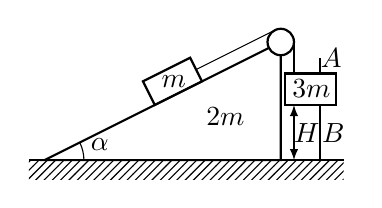
\begin{tikzpicture}
	\coordinate (A) at (0.5, 0);
    \coordinate (B) at (3.5, 0);
    \coordinate (C) at (3.5, 1.5);
       
	\draw [draw=none, pattern=north east lines] (0.3,-0.25) rectangle (4.3, 0);	
	\draw [thick] (0.3, 0) -- (4.3, 0);

	\draw [thick] (A) -- (B) -- (C) node [left=20pt,below=20pt] {$2m$}-- cycle;
	\draw [thick] (1.9,0.7) -- (2.5, 1.0) -- (2.35,1.3) -- (1.75, 1.0) node [right=3pt] {$m$} --  cycle;	
	\draw (2.425,1.15) -- (3.425,1.65);
	\draw [thick, fill=white] (3.5, 1.5) circle (0.168);
	\draw (3.668,1.5) -- (3.668, 1.1);
	\draw [thick] (3.55, 1.1) -- (4.2, 1.1) -- (4.2, 0.7) -- (3.55, 0.7) node [above=6pt,right=-1pt] {$3m$} -- cycle; 
		
	\pic [draw, -, angle eccentricity=1.5] {angle = B--A--C};
	\node [right=20pt, above] at (A) {$\alpha$};
	
	\draw [arrows={latex-latex}] (3.668, 0) -- (3.668, 0.7) node [midway, right=-3.5pt]  {$H$};
	\draw [thick] (4.0, 0) -- (4.0, 0.7) node [midway, right=-3pt] {$B$};
	
	\draw [thick] (4.0, 1.1) -- (4.0, 1.3) node [right=-3.5pt] {$A$};	

\end{tikzpicture}
\end{document}